\documentclass[11pt]{article}
\usepackage{acl2016}
\usepackage{amsmath}
\usepackage{paralist}
\usepackage{subfig}
\usepackage{times}
\usepackage{latexsym}
\usepackage{graphicx}
\usepackage{url}
\usepackage{pgfplotstable}
%\usepackage{hyperref}
\usepackage{color}
\usepackage{lipsum,adjustbox}
\listfiles

\newcommand{\com}[1]{}
\newcommand{\secref}[1]{Section~\ref{#1}}
\newcommand{\figref}[1]{Figure~\ref{#1}}
\newcommand{\tabref}[1]{Table~\ref{#1}}
\newcommand{\XXX}[1]{{\color{red}XXX #1}} % a general todo or comment
%\newcommand{\XXX}[1]{}
\newcommand{\oa}[1]{\footnote{\color{red}OA: #1}}
%\newcommand{\oa}[1]{}
\newcommand{\bh}[1]{\footnote{\color{blue}BH: #1}}
%\newcommand{\bh}[1]{}

\def\perscite#1{\newcite{#1}}
\def\parcite#1{\cite{#1}}
\def\inparcite#1{\newcite{#1}}

\def\equo#1{``{#1}''}  % curly quotes

\newcommand\BibTeX{B{\sc ib}\TeX}

\listfiles

% better maths typography
\def\setsize#1{\lvert #1 \rvert}
\def\func#1{\text{\it #1}}  % much better kerning within function names
\def\HUME{\func{HUME}}
\def\Correct{\func{Correct}}
\def\Partial{\func{Partial}}
\def\Units{\func{Units}}


\title{HUME: Human UCCA-Based Evaluation of Machine Translation}

\author{Author 1\\
	    XYZ Company\\
	    111 Anywhere Street\\
	    Mytown, NY 10000, USA\\
	    {\tt author1@xyz.org}
	  \And
	Author 2\\
  	ABC University\\
  	900 Main Street\\
  	Ourcity, PQ, Canada A1A 1T2\\
  {\tt author2@abc.ca}}

\date{}

\begin{document}

\maketitle

\begin{abstract}
  
%  Recent interest in semantics-aware MT systems underscores the importance of
%  semantic evaluation for Machine Translation (MT) systems. 
%  A semantic measure, sensitive to possible semantic discrepancies
%  between the translation output and the source, is likely to support the construction
%  and tuning of semantics-based MT, much in the same way that string-based measures,
%  such as BLEU, enabled progress in shallower MT.
%  We present a novel human semantic evaluation measure for MT, Human
%  UCCA-based MT Evaluation (HUME), building on the UCCA semantic representation scheme.
%  Making progress over previous work, the proposed measure takes into account
%  a wider range of semantic phenomena and does not rely on semantic annotation
%  of the MT output itself, whose interpretation is often unclear.
%  We experiment with four language pairs, demonstrating HUME's broad applicability,
%  as well as its reliability, reflected in its inter-annotator agreement rates.


Human evaluation of machine translation is a cognitively difficult task and when
annotators rate or rank complete sentences, we see low levels of agreement especially
for longer sentences.  
%In order to extract more reliable annotations, previous research broke down evaluation into smaller components by asking humans to annotate semantic roles on the source and translation, and then to align them. 
In order to extract more reliable annotations, previous research broke down
evaluation into smaller components in various ways. 
We propose a new evaluation method, HUME, 
which is based on the Universal Conceptual Cognitive Annotation (UCCA)
semantic annotation.
UCCA is applicable across many languages, it has better coverage of important
semantic phenomena than previously used semantic annotation,
semantic role labeling, and it is grounded in the words in the sentence. 
We apply UCCA only over the source or reference sentence, and not over the
possibly garbled translation.
%, 
%and this makes annotation more reliable and also efficient as we can reuse labor
%intensive semantic annotations.
We show that HUME can be reliably applied to
four different target languages and that sentence-level inter-annotator agreement
does not decrease over longer sentences. 

\end{abstract}


%%%%%%%%%%%%%%%%%%%%%%%%%%%%%%%%%%%%%%%%%%%%%%%%%%%%%%%%%%%%%%%%%%%%%%%%%%%%%%%%%%%%%%
\section{Introduction}\label{sec:intro}

Human judgement is the central, and perhaps most fundamental, criterion for
estimating the quality of an MT system.
Nevertheless, common measures for MT evaluation, such as adequacy and fluency judgements
or the relative ranking of several possible translations, are problematic in two ways.
First, as the quality of translation is determined by multiple factors, it is difficult
to assign a single number that quantifies the quality of the entire sentence. This
is indeed reflected in the diminishing inter-annotator agreement (IAA) rates of human ranking measures
%as a function of
with
the sentence length \cite{Bojar:2011}.
Second, a sentence-level quality score does not indicate what parts of the sentence
are erroneously translated, and hence cannot inform developers in overcoming these errors.

These problems are partially addressed by measures that decompose over sub-parts of the evaluated
translation sentence (henceforth, {\it translation}). For automatic measures,
these are commonly words or n-grams, for manual measures some structural
information is taken into account \parcite{machacek:bojar:segranks:2015}.
% the following is specific to automatic measures:
%quantifying the overlap of its sub-parts relative a reference translation.
A promising line of research decomposes
%More recent work on MT evaluation proposed measures
%that decompose
over semantically defined units,
quantifying the similarity of the output and the reference in terms of
their verb argument structure; the most notable of these measures is
HMEANT \cite{lo2011structured}.
\XXX{Do we want to cut the following shorter?}
These measures can localize semantic errors in the translation, but
their focus on verb argument structures misses many pervasive semantic phenomena
(such as inter-clause linkage and nominal argument structures) and thus they only provide
a limited perspective on the semantic similarity between the output and reference.
Moreover, assigning semantic structure to MT output, especially when low in quality,
is difficult and arguably ill-defined.

We propose the Human UCCA-based MT Evaluation (HUME) metric,
a human evaluation measure that decomposes over the semantic units of the sentence.
Semantic units are defined according to the 
UCCA scheme \cite{abend2013universal}, an appealing candidate for semantic analysis,
due to its cross-linguistic applicability, support for rapid annotation, and coverage
of many fundamental semantic phenomena, such as verbal, nominal and adjectival
argument structures and the inter-relations between them.

HUME operates by aggregating human assessments of the translation quality of individual
semantic units in the source sentence.
Importantly, HUME only requires semantically annotating the source sentence,
thus avoiding the annotation of machine-generated text 
and allowing re-use of the source semantic annotation for measuring the quality
of different translations of the same source sentence.
By basing the measure on a direct comparison
of the source and translation we avoid the difficulties engendered by using
reference translations, albeit at the cost of imposing the additional requirement
that the evaluator be proficient in both the source and target languages.
%An elaborate comparison of HUME and HMEANT is given in \secref{sec:hmeant_comp}.

After a brief review (\secref{sec:background}), we describe HUME in detail
(\secref{sec:hume}) and highlight its benefits over HMEANT
(\secref{sec:hmeant_comp}).
Our experiments with four language pairs: English-German, English-Polish,
English-Romanian and English-Czech (\secref{sec:experiments}) document the
efficiency (time of annotation) and inter-annotator agreement scores for HUME.

% We conduct experiments with four language pairs: English-German, English-Polish,
% English-Romanian and English-Czech, and report efficiency (time of annotation) and
% inter-annotator agreement scores (\secref{sec:experiments}).
% 
% \XXX{The following should go rather to the conclusion}
% Efficiency results that HUME
% can be annotated in 2--4 minutes, once the UCCA annotation of the source is given,
% which is only about five times slower than MEANT, and hence still practical to
% employ on a moderate scale. HUME's agreement results are on par with those
% of standard sentence-level ranking measures, but unlike them,
% HUME's scores do not decrease with longer sentences.\bh{We may
%   have to focus more on qualitative aspects, if we just try to sell
%   the measure on IAA, then the figures are not stunning. OA: is that OK?}



%%%%%%%%%%%%%%%%%%%%%%%%%%%%%%%%%%%%%%%%%%%%%%%%%%%%%%%%%%%%%%%%%%%%%%%%%%%%%%%%%%%
\section{Background}\label{sec:background}

%While the measure addresses the two major shortcomings 
%detailed above, it is unable to capture semantic differences which do not show up in 
%the verb-argument structure, including several very frequent phenomena, 
%Another shortcoming of MEANT is its reliance on semantically annotating MT output,
%which is often unintelligible. Finally, measures based on a comparison to a


%These difficulties have motivated the definition of a human measure that decomposes over
%the semantic structure of the sentence, rather than its n-grams. The most notable attempt of
%this type is the MEANT measure, and its human variant HMEANT
%\cite{lo2010evaluating,lo2011structured,Lo2011meant,lo2013meant}, which quantifies the
%similarity between the output translation and a reference translation in terms of the similarity
%between their verbal argument structures
%While the measure addresses the two major shortcomings
%detailed above, it is unable to capture semantic differences which do not show up in
%the verb-argument structure, including several very frequent phenomena, such as
%inter-clause linkage, nominalizations and copula clauses
%(see \secref{sec:hmeant_comp}).
%Another shortcoming of MEANT is its reliance on semantically annotating MT output,
%which is often unintelligible. Finally, measures based on a comparison to a
%reference translation
%are necessarily incomplete, as they compare to a small number of references
%out of the the huge number of possible translations a sentence may have
%\cite{dreyer2012hyter}.


\paragraph{Machine Translation Evaluation.}
%MT evaluation has been traditionally pursued through human-based
%evaluation that quantifies the adequacy of the translation in preserving the meaning 
%of the source sentence, and its fluency as a sentence in the target language \cite{lopez2008statistical}.
Human evaluation is generally done by ranking the outputs of multiple systems
e.g., in the WMT shared tasks \cite{bojar2015findings}, or by assigning
individual adequacy/fluency scores to each translation, a procedure recently improved
by \newcite{graham2015improving}.
However, while providing the gold standard for MT evaluation, human evaluation
is not a scalable solution.
%and is infeasible where a wide variety of systems or parameter settings are to be evaluated.
% has motivated the construction of cheaper methods that correlate with human
%judgement.

Scalability is addressed by employing automatic and semi-automatic approximations of human
judgements. Commonly, such scores decompose over the sub-parts of
the translation, and quantify how many of these sub-parts appear in a manually created reference translation.
This decomposition further allows system developers
to localize the errors, or at least unconfirmed parts within the translation.
The most commonly used measures decompose over n-grams or individual words, e.g., 
BLEU \cite{Papineni:2002}, NIST \cite{Doddington:2002} and METEOR  \cite{Banerjee:2005}.
Another common approach is to determine the similarity between the reference and translation
by applying string edit distance \cite{snover2006study}.
While these measures stimulated much progress in MT research by allowing
the evaluation of massive-scale experiments,
their decomposition over words and n-grams is better suited for localizing errors
in the output of shallow MT methods, and is less instructive in identifying the semantic
nature of the errors. 

%These methods are most suitable for evaluating shallow MT approaches and are
%less instructive as to what aspects of the reference's meaning were not preserved
%in the translation output.
%A common approach is to compare the MT output with reference translations,
%created or verified by an expert. Methods often rely on some sort of string matching
%methods, such as overlap of n-grams, as with the BLEU and METEOR measures, or edit
%distance.
%First, they rely on comparison to reference translations, which reflect a small
%number out of the enormous number of ways to translate a sentence and are thus
%inherently incomplete. 

In order to address this shortcoming, more recent work quantified
the similarity of the reference and translation in terms
of their structure. \newcite{liu2005syntactic} took a syntactic approach, 
quantifying the similarity between the syntactic structures of the reference and translation.
\newcite{owczarzak2007evaluating} took a similar approach using lexical-functional grammar structures.
\newcite{gimenez2007linguistic} proposed to aggregate multiple types of information,
capturing the overlap between the output and reference in terms of their
semantic (predicate-argument structures), lexical and morphosyntactic features.

Perhaps the most notable attempt at semantic MT evaluation is MEANT and
its human variant HMEANT \parcite{lo2011structured}, which quantifies the similarity between
the reference and translation in terms of the overlap in
their verbal argument structures structures and associated semantic roles.
We discuss the differences between HMEANT and HUME in \secref{sec:hmeant_comp}.

%\begin{figure}
%
%\begin{tikzpicture}[semithick, x=2.4cm,y=0.8cm, >=latex, baseline=7ex,
%    inner sep=.3ex, outer sep=.7ex, minimum size=1.2ex,->]
%  \node (ROOT) [fill=black, circle] {}
%  child {node {After} edge from parent node[left]  {$L$\hspace{1.5cm}}}
%  child {node (H1)  [fill=black,circle] {}
%    child {node {graduation} edge from parent node[right] {$P$}}
%      %child {node {to Paris} edge from parent node[right] {$A$}}
%      edge from parent node[left] {$H$}
%    }
%    child {node (H2)  [fill=black,circle] {}
%      child {node  {} edge from parent[draw=none]}
%      child {node  {} edge from parent[draw=none]}
%      child {node  (Tom) {Tom} edge from parent node[right] {$A$}}
%      child {node  {moved} edge from parent node[right] {$P$}}
%      child {node  [fill=black,circle] {}
%        child {node  {to} edge from parent node[right] {$R$}}
%        child {node  {NYC} edge from parent node[right] {$C$}}
%        edge from parent node[right] {$A$}}
%      %child {node {to Paris} edge from parent node[right] {$A$}}
%      edge from parent node[left] {$H$}
%    };
%    \draw (H1) -> (Tom) node[midway, right] {$A$ \hspace{0.2cm}};
%  \end{tikzpicture}
%\caption{\label{fig:ucca_example}
%  Sample UCCA annotation of the sentence ``After graduation, Tom moved
%  to NYC''. Leaves correspond to words, whereas nodes correspond to units.
%  Edge labels mark UCCA categories, which are described in the table.}
%%which are largely ignored in this work
%\end{figure}


\begin{figure}
    \begin{center}
    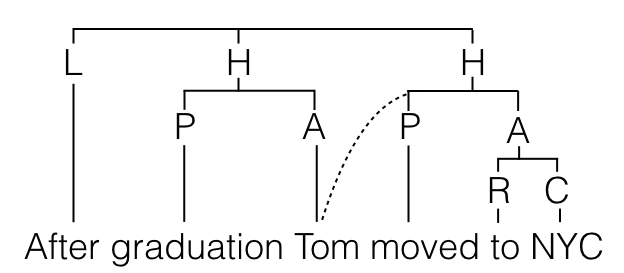
\includegraphics[width=0.45\textwidth]{ucca-tree-v2.png}

\begin{tabular}{|l|l|l|l|}
\hline
L & Linker &  A & Participant \\
H & Scene & R & Relator \\
P & Process & C & Centre \\
\hline
\end{tabular}
    \end{center}
\caption{\label{fig:ucca_example_v2}
  Sample UCCA annotation where leaves correspond to words and nodes correspond to units.
  Edge labels mark UCCA categories, which are described in the table.}
%which are largely ignored in this work
\end{figure}

\paragraph{Semantic Representation.}
UCCA (Universal Conceptual Cognitive Annotation, \inparcite{abend2013universal}) is a
cross-linguistically applicable, lightweight
scheme for semantic annotation. Formally, a UCCA structure is a directed acyclic graph (DAG),
whose leaves correspond to the words of the text.
The graph's nodes, called {\sc units}, are either terminals or several elements jointly
viewed as a single entity according to some semantic or cognitive consideration. Edges bear
a category, indicating the role of the sub-unit in the structure the unit
represents.

UCCA's current inventory of distinctions focuses on argument structures
(adjectival, nominal, verbal and others) and relations between them.
The most basic notion is the Scene, which describes a movement, an
action or a state which is persistent in time. Each Scene contains one main relation, as well
as one or more participants. For example, the sentence ``After graduation, Tom moved to NYC''
contains two Scenes, whose main relations are ``graduation'' and ``moved''.
The participant ``Tom'' is a part of both Scenes, while ``NYC'' only of the
latter (\figref{fig:ucca_example}). Further categories account for
relations between Scenes and the internal structures of complex participants and relations.

% UCCA Motivation
UCCA is a natural candidate for defining a semantic
MT evaluation measure for a number of reasons. 
First, it defines an intuitive set of categories
that can be reliably annotated by non-experts, after as little as two hours
of training \cite{marinotti2014}.
Second, UCCA is a cross-linguistically applicable scheme, seeking to
represent what is shared between languages
by building on linguistic typological theory, and specifically on ``Basic Linguistic Theory''
\cite{Dixon:10a,Dixon:10b,Dixon:12}, one of the most widely used frameworks for linguistic description.
The cross-linguistic applicability of UCCA has been tested in annotations of
English, French, German and Czech.
Third, the scheme has been shown to be semantically stable
in translation: UCCA annotations of translated text usually contain the same set of relationships
\cite{sulem2015conceptual}. This is an indication that the scheme reflects
a common layer of representation that in a correct translation
is mostly shared between the translation and the source. 

We note that verbal argument structures are less stable in this sense, as a verbal
argument structure may be translated or paraphrased to a nominal or adjectival
argument structure, and are thus less suitable as a basis for a semantic measure.
E.g., ``after he graduated, Tom moved to NYC'' contains two verbs,
but is similar in meaning to the one-verbed
``after graduation, Tom moved to NYC''. 

% While most broad-coverage semantic work focused on shallow semantic structures,
% predominantly argument structures annotated with their semantic roles, much recent
% interest has been devoted to defining more complete semantic representation schemes.
% \oa{should we
% add that it is less cross-linguistically stable? maybe that's an overkill..
%  OB: AMR has been applied to more languages, including Chinese, so I would not
%  dare saying that it is less stable.}

The Abstract Meaning Representation (AMR) scheme \cite{banarescu2013abstract}
shares much of UCCA's motivation for defining a more complete semantic annotation.
However, using AMR is not optimal for defining a decomposition of a sentence into semantic
units as it does not ground its semantic symbols in the text,
thus does not provide clear decomposition of the sentence into sub-units.
Also, AMR is more fine-grained than UCCA and consequently more difficult to annotate.
Other approaches pursued a grounded representation of semantics,
and have generally represented semantic structures as bi-lexical dependencies.
Examples include the tectogrammatical layer \parcite{sgallhp:1986} used in the Prague dependency
treebanks, e.g. the Czech-English one \parcite{hajic2012announcing}, as well
as dependencies derived from Minimal Recursion Semantics representations \parcite{oepen2006discriminant}.
Nevertheless, despite their appeal as deep and intuitive means for semantic representation,
these approaches require linguistic expertise for their annotation, due to the intricate and
fine-grained distinctions they provide, and are thus in our view less suitable for basing
an interpretable MT evaluation on. 

%\newcite{Basile:12} attempted to make some aspects of the semantic annotation more accessible,
%but to our knowledge no results of this brand have been reported.


%%%%%%%%%%%%%%%%%%%%%%%%%%%%%%%%%%%%%%%%%%%%%%%%%%%%%%%%%%%%%%%%%%%%%%%%%%%%%%%%%%%
\section{The HUME Measure}\label{sec:hume}


\subsection{Annotation Procedure}\label{sec:guidelines}

This section summarises the manual annotation procedure performed in order 
to compute the HUME measure. 
We mark the source sentence as $s$ and the translation sentence as $t$. 
The procedure involves two manual steps: (1) UCCA-annotating $s$, 
(2) human judgements as to the translation quality of each semantic unit of $s$ relative to $t$,
where units are defined according to the UCCA annotation.
We note that UCCA annotation is performed once for every source sentence,
irrespective of the number of its translations we wish
to evaluate\footnote{Instead of relying on the source,
the evaluation could be based on the UCCA structure for the \emph{reference}
translation. This would allow monolingual annotators to take part in the
evaluation. On the downside, the translation would have to be aligned to the
reference and more importantly, we would risk inaccurate judgements due to
the naturally occurring differences between the source and its reference
translations.}.

\paragraph{UCCA Annotation.}
We begin by creating UCCA annotations for the source sentence, following the
UCCA guidelines\footnote{All UCCA-related resources can be found
  here: \url{http://www.cs.huji.ac.il/~oabend/ucca.html}}.
Let $L$ be the set of possible UCCA labels.
Given a sentence $s = (w_1, \ldots,w_n)$, its UCCA annotation is a DAG $G=(V,E,\ell)$,
where $\ell: V \rightarrow L$, and where $W = \{w_1,\ldots,w_n\}$ correspond to the leaves of $G$.
For every node $v \in V$, we define its {\it yield} $yld(v)$ as $v$'s descendants in $W$.
The semantic units for a sentence $s$ according to $G$
is the set of yields of nodes in $V$. 
We note that the translation is not UCCA-annotated.

%\begin{figure*}[t]
%    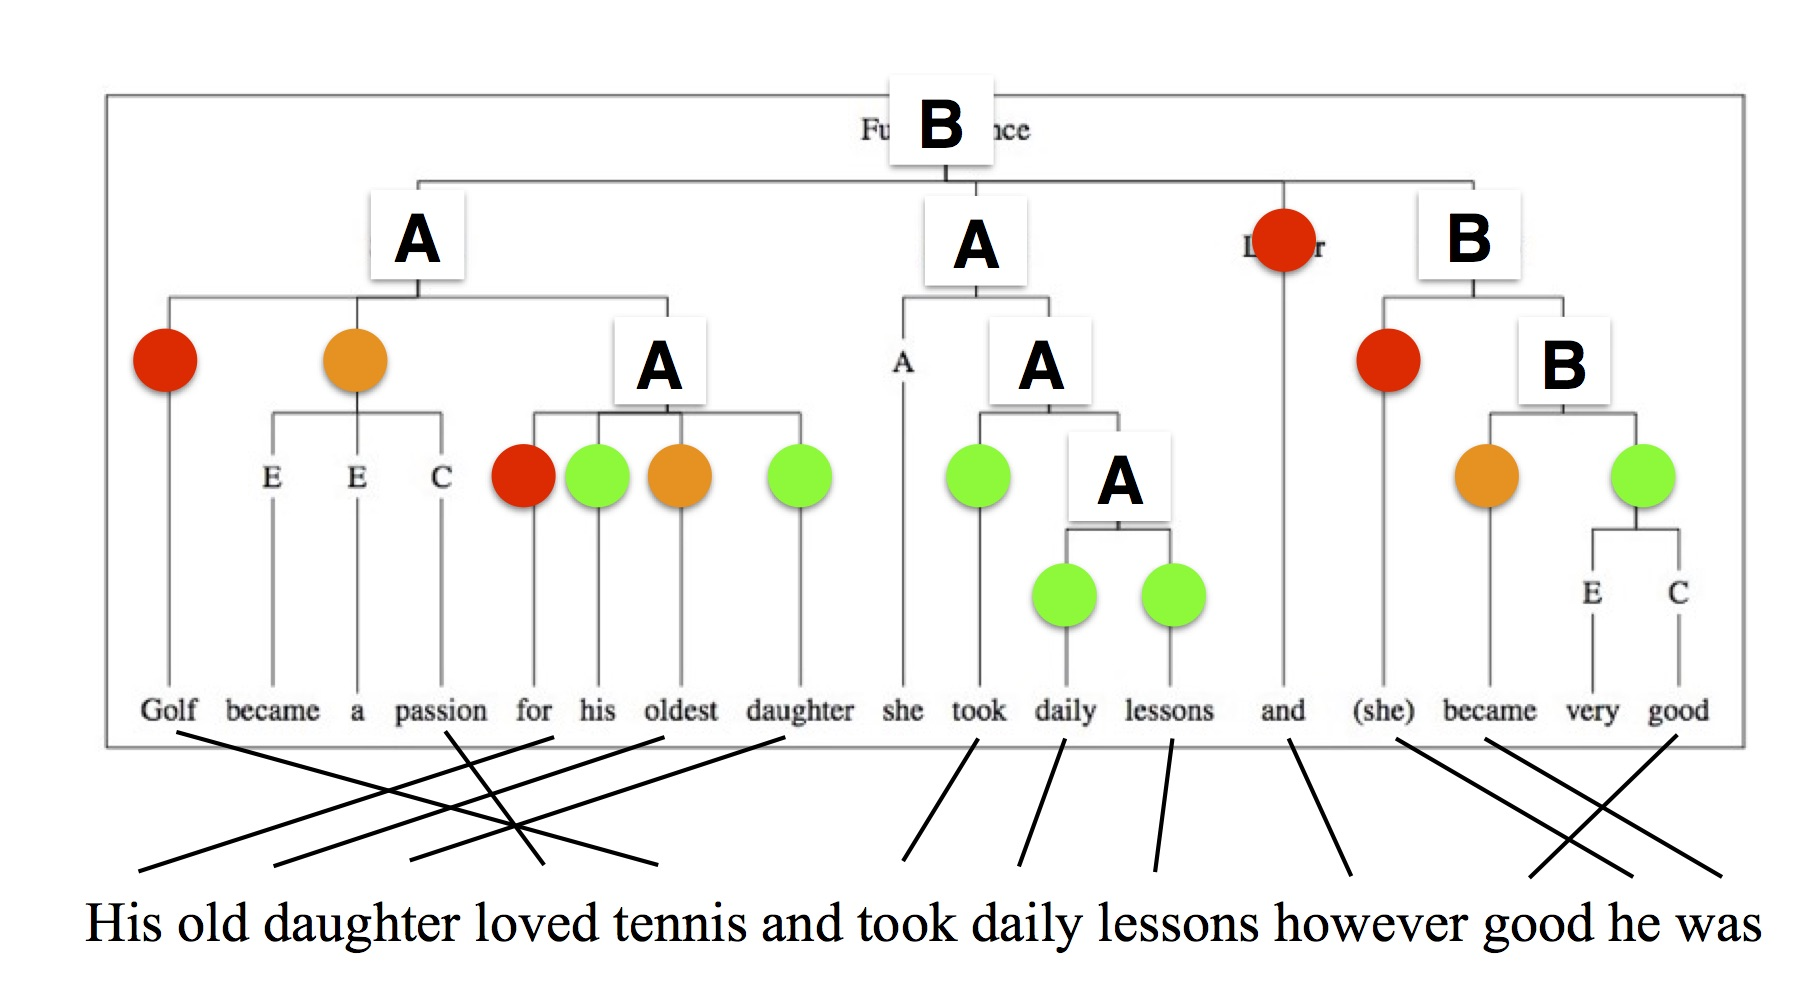
\includegraphics[width=1\textwidth]{ucca-tree-mteval.jpg}
%    \caption{UCCA Tree evaluated in comparison to an aligned ``translation'' (an
%	English paraphrase).}
%    \label{fig:ucca-tree-hume}
%\end{figure*}

\begin{figure}
    \begin{center}
    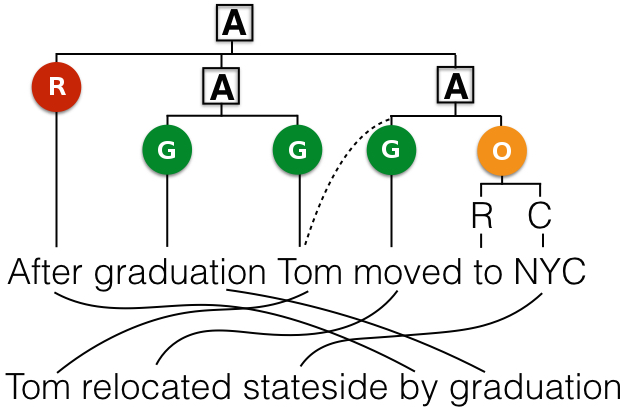
\includegraphics[width=0.45\textwidth]{ucca-tree-mteval-v2.png}
    \end{center}
  \caption{\label{fig:hume_tree_v2}
     HUME annotation of an UCCA tree with a word aligned example translation shown below. 
Atomic units are labelled using traffic lights and structural nodes are marked A or B.}
\end{figure}

In Figure~\ref{fig:hume_tree_v2} we can see an example of a possible HUME
annotation, with the translation shown in English for ease of comprehension.
When evaluating ``to NYC'' the annotator looks at the translation and sees the
word ``stateside''. This word captures the whole phrase and so we mark the
structural node with an atomic label. Here we choose ``Orange'' but the
annotator could equally have decided that this translation is wrong and marked
it as ``Red''. The ability to mark structural nodes with atomic labels allows
the annotator to account for translations which only correspond at the phrase
level. Another feature highlighted in this example is that the root node is
``Adequate''. This might seem confusing, as the relationship between the scenes
has changed in the translation. However, an important feature of HUME is that
penalises errors where they occur. In HUME, the error is caused by a wrong
translation of the linker ``After'' which translates as ``by'' and this is
marked as ``Red''. The root node still has two scenes linked by one linker and
the relationship between child nodes is maintained and therefore it is marked
``Adequate''.
% Ondrej removes the following, he thinks that errors are not supposed to be
% propagated in HMEANT either:
%In HMEANT, it is not clear whether errors should be propegated up the SRL hierarchy. 



%\begin{figure*}
%  \begin{adjustbox}{trim=2.3cm 0 0 0}
%   \begin{tikzpicture}
%     [ level distance=12mm,
%	   level 1/.style={sibling distance=7.5em,level distance=7mm},
%       level 2/.style={sibling distance=5em,level distance=12mm},
%       level 3/.style={sibling distance=5em},
%       level 4/.style={sibling distance=3em}]
%     %[semithick, x=2.4cm,y=0.8cm, >=latex, baseline=7ex,
%     %  inner sep=.3ex, outer sep=.7ex, minimum size=1.2ex,->]
%   \node (ROOT) [label={B}] [fill=blue, circle] {}
%   child {node (H3) [label={A}] [fill=yellow,circle] {}
%     child {node [label={[red]:R}] {Golf} edge from parent node[left] {}}
%     child {node (H1) [label={[orange]30:O}] [fill=orange,circle] {}
%       child {node [label={}] {became} edge from parent node[left]  {}}
%       child {node [label={}] {a} edge from parent node[left]  {}}
%       child {node [label={}] {passion} edge from parent node[left]  {}}
%     }
%     child {node (H2) [label={A}] [fill=yellow,circle] {}
%       child {node {} edge from parent[draw=none] {}}
%       child {node {} edge from parent[draw=none] {}}
%       child {node {} edge from parent[draw=none] {}}
%       child {node {} edge from parent[draw=none] {}}
%       child {node [label={[red]:R}] {for} edge from parent node[left]  {}}
%       child {node [label={[green]:G}] {his} edge from parent node[left]  {}}
%       child {node [label={[orange]:O}] {oldest} edge from parent node[left]  {}}
%       child {node [label={[green]:G}] {daughter} edge from parent node[left]  {}}
%     }
%   }
%   child {node {} edge from parent[draw=none] {}}
%   child {node (H4) [label={[]30:A}] [fill=yellow,circle] {}
%     child {node (she) [label={[green]:G}] {she} edge from parent node[left]  {}}
%     child {node [label={[green]:G}] {attended} edge from parent node[left]  {}}
%     child {node [label={[green]:G}] {daily} edge from parent node[left]  {}}
%     child {node [label={[green]:G}] {lessons} edge from parent node[left]  {}}
%   }
%   child {node [label={[red]:R}] {and} edge from parent node[left]  {}}
%   child {node (H5) [label={A}] [fill=yellow,circle] {}  
%     child {node [label={[red]:R}] {greatly} edge from parent node[left] {}}
%     child {node [label={[orange]:O}] {improved} edge from parent node[left] {}}
%   };
%   \draw[dashed] (H5) -> (she) ;
% 
%   \com{
%   child {node (H1) [label={\#8}] [fill=black,circle] {}
%     child {node [label={\#2}] {graduation} edge from parent node[right] {$P$}}
%       %child {node {to Paris} edge from parent node[right] {$A$}}
%       edge from parent node[left] {$H$}
%     }
%     child {node (H2) [label={\#9}] [fill=black,circle] {}
%       child {node  {} edge from parent[draw=none]}
%       child {node  {} edge from parent[draw=none]}
%       child {node [label={\#3}] (Tom) {Tom} edge from parent node[right] {$A$}}
%       child {node [label={\#4}] {moved} edge from parent node[right] {$P$}}
%       child {node [label={\#10}] [fill=black,circle] {}
%         child {node [label={\#5}] {to} edge from parent node[right] {$R$}}
%         child {node [label={\#6}] {NYC} edge from parent node[right] {$C$}}
%         edge from parent node[right] {$A$}}
%       %child {node {to Paris} edge from parent node[right] {$A$}}
%       edge from parent node[left] {$H$}
%     };
%     \draw (H1) -> (Tom) node[midway, right] {$A$ \hspace{0.2cm}};
%     }
%   \end{tikzpicture}
%  \\
%  \end{adjustbox}
%    % Ondrej removed the width=\textwidth from the options below to keep font
%	% unenlarged:
%  \adjustbox{center,margin=.5em}{\it His old daughter loved tennis, and took daily lessons however good he was}
%
%  \caption{\label{fig:hume_tree}
%    Sample UCCA annotation of a source sentence, translation (below in italics), 
%    and translation judgements over the source units, marked with A,B,R,O,G labels. Yellow/blue marks
%    nodes annotated with A/B, respectively.
%    In our experiments, the translation is in German, Romaninan, Polish or Czech.
%    ``became a passion'' is marked as atomic, as it is a multi-word expression.
%    The dashed line indicates that ``she'' is also a child of the unit ``greatly improved''.
%    UCCA categories, and alignment between source and translation are omitted for brevity.}
%  
%\end{figure*}


\paragraph{Translation Evaluation.}
The basic strategy for computing HUME is to traverse the semantic units
of the source sentence, which correspond to the different arguments and relations expressed
in the text, and to mark the extent to which they have been correctly translated.
HUME aggregates the judgements of the users into a composite score, 
which reflects the overall extent to which the semantic content of $s$ is preserved in $t$.

Human annotation of the semantic units requires first deciding whether
a unit is {\it structural}, i.e., has meaning-bearing sub-units,
or {\it atomic}. In most cases, atomic units
correspond to individual words, but they may also correspond to unanalyzable
multi-word expressions, i.e., expressions that do not have meaningful sub-units
(e.g., idioms like ``takes two to tango'').
When a multi-word unit is labeled as atomic, all its sub-units' annotations are discarded
from the evaluation.

Atomic units can be labelled as ``Green'' (correct), ``Orange'' (partially correct)
and ``Red'' (incorrect). 
A Green label means that the meaning of the word or phrase has been largely preserved.
An Orange label means that the essential meaning of the unit has been preserved,
but some part of the translation is wrong.
This could often be due to the translated word having the wrong tense,
or the wrong morphology, in a way that impacts little on the understandability of the sentence.
A Red label means that the essential meaning of the unit has not been captured.

Structural units have sub-units (children in the UCCA graph), which may themselves
either be atomic or structural. The labels assigned to such nodes reflect the extent to which
the relation between the sub-units is preserved in $t$.
For instance, a Scene unit represents the relation between the
Scene elements, such as the predicate (main relation), participants and adverbials.
Structural units are labeled as ``Adequate'' or ``Bad'', meaning
that the relation between the sub-units went wrong.
We use a three label system with atomic units, as
opposed to a two label one in structural units,
as atomic units often have slight errors, in which cases we do want to provide partial credit.

There are many ways that the relationship between the children might go
wrong in translation

\begin{compactitem}
\item The components of the translation are ordered differently from the source,
  such that the relation between them changes. For instance, where
  the sentence ``man bites dog'' is translated into a sentence meaning ``dog bites man'',
  the semantic unit corresponding to the Scene will be marked as Bad, while
  the individual atomic units ``dog'', ``bites'' and ``man'' will be marked as Green.
\item A superfluous word or phrase has been inserted into
  the translation. For instance, if ``dog bites man'' is translated into ``dog viciously bites man''.
\item One of the sub-units is missing from the translation.
  For instance, if ``dog bites man'' is translated into ``dog bites''. \bh{Note that in this case we also 
  get an error in the atomic unit, assuming that ``man'' is a semantic unit in the source, but for the other
  two cases there is no atomic unit error.}
\end{compactitem}

We note that HUME labels reflect adequacy, rather than fluency judgements.
Specifically, annotators are instructed to
label a unit as Adequate if its translation is understandable and preserves
the meaning of the source unit, even if its fluency is impaired.

In non-configurational languages, the relationship between the
governing and the dependent units is often expressed using morphological
properties of the dependents instead of their ordering
(this holds especially for the verb and its modifiers,
less so for components of noun phrases). Since errors in morphology
should be expressed on the atomic units, we would expect
a higher proportion of ``Adequate'' structural units for Czech and Polish
compared to German and Romanian\oa{but doesn't German also have a case system? Ondrej:
  could you pinpoint what the difference exactly is?}.

An example HUME annotation is given in \figref{fig:hume_tree},
which presents an annotation of an UCCA tree, and a corresponding translation.
We see that ``became a passion'' is deemed atomic, as it is translated as a single unit
in $t$, and thus its sub-units, ``became'', ``a'' and ``passion'' are not evaluated
individually. 

%For example, consider the sentence ``After graduation, Tom moved
%to NYC'' as the source $s$, see \figref{fig:ucca_example}.
%The atomic units are the individual words,
%nodes \#1--6 and the structural nodes are \#7--10. Assume that the translation $t$
%is ``After Tom will move to Paris, graduation''\footnote{We take $t$ to
%  be in English for presentation purposes. In our experiments, $t$ is in German,
%  Czech, Polish or Romanian.}.
%Then ``after'', ``graduation'', ``Tom'' and ``to'' are marked Green, ``moved'' is marked
%Orange (as it corresponds to ``will move'' in $t$), and ``NYC''
%is marked as Red, as it was mistranslated to ``Paris''. Node \#9 is marked Adequate,
%as the Scene of Tom moving is properly reflected in the translation. Node \#10, which
%expresses the relation between the graduation and moving Scenes, is marked Bad,
%as their relation in $t$ is reversed.


\subsection{Composite Score}\label{sec:score}

We proceed to detailing how judgements on the semantic units
of the source are aggregated into a composite score.
While future extensive empirical evaluation with HUME and its application to MT
system tuning may suggest more complex definition,
as a starting point we take a parsimonious approach,
and compute an accuracy score.

Let $\Correct(s,t)$ be the number of atomic units in $s$ marked as Green relative to $t$ plus
the number of structural units in $s$ marked as Adequate relative to $t$.
Let $\Partial(s,t)$ be the number of atomic units in $s$ marked as Orange relative
to $t$. Let $\Units(s)$ be the total number of units marked with any of the five labels.
Then HUME's composite score is:

\vspace{-.5cm}
\begin{equation}
  \small
  \HUME(s,t) = \frac{\Correct(s,t) + 0.5\cdot \Partial(s,t)}{\setsize{\Units(s)}}
  \nonumber
\end{equation}



%%%%%%%%%%%%%%%%%%%%%%%%%%%%%%%%%%%%%%%%%%%%%%%%%%%%%%%%%%%%%%%%%%%%%%%%%%
\subsection{Annotation Interface}

We turn to discuss the interface for collecting human judgements on the semantic units
of the source, relating to the translation. UCCA annotations of the source are done offline,
using the UCCA web application.

\figref{fig:interface} presents the user interface of HUME. 
The translation appears at the top, and
the source sentence directly below it. Underneath the source sentence appears
its list of semantic units. For each semantic unit, including the one for the
entire source sentence, there is a textbox, displaying the yield of that unit.
Information on the category of the unit (e.g., whether it is a Scene, participant etc.).
The user is asked to select a label for each unit,
by clicking the ``A'', ``B'', Green, Orange, or Red buttons to the left of the unit's box.

The interface presents, for each unit, the translation segment aligned with it.
This allows the user, especially in long sentences, to focus her attention on the parts
most likely to be relevant for her judgement. As the alignments are automatically derived,
and therefore noisy, the annotator is instructed to treat the aligned text is a cue, but to ignore
the alignment if it is misleading, and instead 
make a judgement according to the full translation sentence.

Concretely, let $s = (w_1,\ldots,w_n)$ be a source sentence, $t = (w'_1,\ldots,w'_n)$ a translation,
and $A \subset 2^{s \times t}$ a many-to-many word alignment between them.
If $u$ is a semantic unit in $s$, whose yield is $yld(u)$, we define the aligned text in
$t$ to be $a(u)=\bigcup_{(x_s,x_t) \in A \wedge x_s \cap yld(u) \neq \emptyset} x_t \subset t$.
Where $a(u)$ is discontiguous in the text, words between the left
and right boundaries of $a(u)$ which are not contained in it (intervening words)
are presented in a smaller red font.
Intervening words are likely change the meaning of the translation
of $u$, and thus should be paid attention to when considering whether the translation
is correct or not.

For example, consider the sentence $s=$``We're driving back on Friday'' and the German
translation t=``Am Freitag fahren wir zur\"uck'' (lit. ``on Friday driving we back'').
``driving back'' will be aligned to ``fahren ... zur\"uck'',
and ``wir'' will be marked as intervening word. Another example
appears in \figref{fig:interface}, where ``ongoing pregnancy'' is translated to
``Schwangerschaft ... laufenden'' (lit. ``pregnancy ... ongoing'').


% Ondrej did the following in a footnote in Section 3.1 Annotation Procedure
%\bh{Somewhere we could explain that we
%could do a similar annotation with monolinguals, although it entails aligning
%reference and MT output}


%There are cases where we cannot usefully compare individual words in the source to words in the target.
%We often need to compare translation at the phrase level. If this is the case, then we can 
% treat the structural node as a lexical unit, and mark it with the traffic light labels. This 
%means that none of the children of this node will be examined in order determine the semantic score
%for this sentence. 
%In Figure~\ref{ucca-tree-mteval}, we can see that the phrase ``became a passion'' has been labelled as a lexical
%node and it has been evaluated as ``Orange'', or partially correct, as the translation of this phrase ``loved'' 
%only partially capture the semantics of the source.


\begin{figure*}[t]
    \begin{center}
    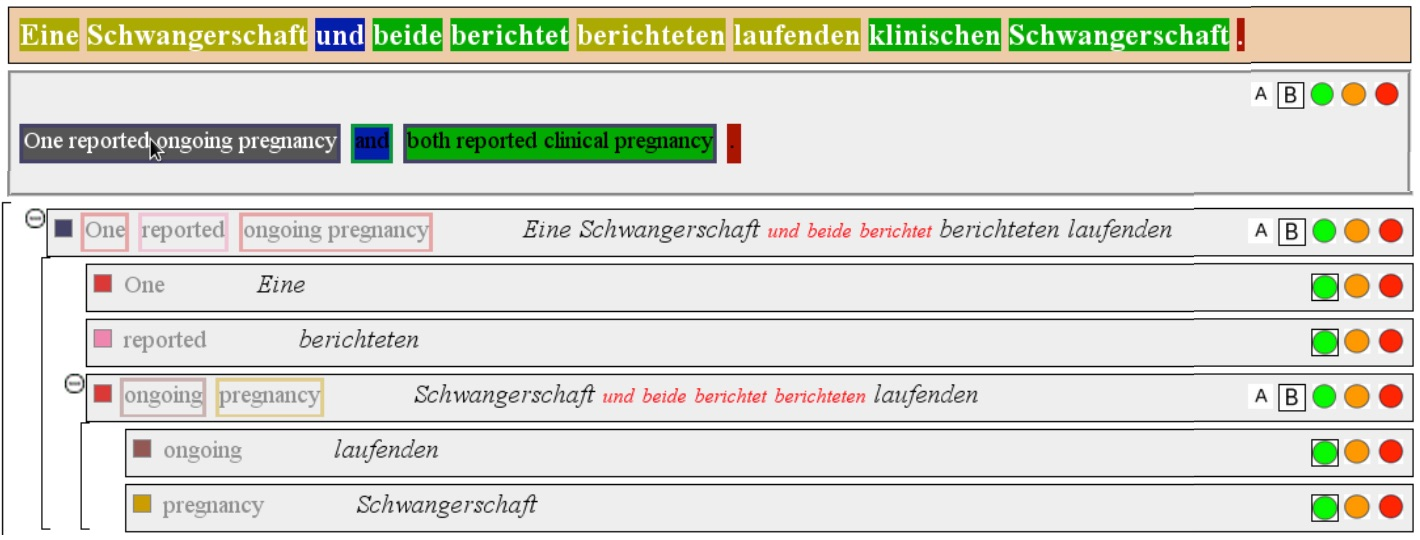
\includegraphics[width=1\textwidth]{hume_interface2.jpg}
    \caption{The HUME annotation tool, based on the UCCA tool. The faded orange box at the top
      presents the translation, the large box below it presents the source. The tree of semantic units
      for the source is given underneath, where the aligned text appears in italics, and intervening words
      appear in red with a smaller font (e.g., in the first box).}
    \label{fig:interface}
    \end{center}
\end{figure*}

\com{
In Figure~\ref{mttool} you we show the MT evaluation tool. The sentence at the top shows the complete MT system output. Underneath the MT output is the  source sentence.  Underneath the source sentence we see its expandable semantic tree structure with both lexical and structural nodes. atomic nodes only have traffic light annotation, whereas a structural node would normally be labelled ``A'' or ``B'' but could also be labelled as a lexical node, in the case where there is no word to word correspondence for the translation of its children.

 The child components of a structural node are marked with different coloured rectangles. When navigating through the different source sentence nodes, one can see the relevant sections of the translation because the aligned words in the translation are highlighted in the complete sentence above. Aligned translations are also shown in black alongside the source node. If the node is aligned to a set of discontiguous words in the translation, then the unaligned words that appear in between the aligned words are shown in red. Even if these words are not directly aligned to the source node, they 
will likely change the meaning of the translation and must be considered when marking 
the translation as correct or not. The alignments are meant just as a guide. The annotator should  look at the complete translation when deciding on the evaluation of a node. The translation could have content added before or after the node which changes its
 structure or meaning. If an extra component is prepended to a structural node, for example, it should be marked as ``Bad''.
}



%%%%%%%%%%%%%%%%%%%%%%%%%%%%%%%%%%%%%%%%%%%%%%%%%%%%%%%%%%%%%%%%%%%%%%%%%%%%%%%%%%%
\section{Comparison with HMEANT}\label{sec:hmeant_comp}

HMEANT shares much of HUME's motivation in defining a
measure that decomposes over semantic units, rather than strings. On the other
hand, there are important differences in design decisions, which we summarize in this
section.

First of all, the annotation process is different. We semantically annotate the
source, then automatically project it to the translation, and ask bilingual
annotators to assess whether this projection shows a good or bad translation. In
HMEANT, they semantically annotate both the reference and the translation, then
align these manually, and assess to what extent they match.


\paragraph{Verbal Structures Only?}

HMEANT focuses on verbal
argument structures, ignoring other pervasive phenomena such as nominal predicates, inter-clause
relations and copula clauses. Some of the uncovered cases were already observed
in previous applications of HMEANT to languages other than English (see \perscite{birch-EtAl:2013:WMT} for German, \perscite{bojar:wu:ssst:2012} for
Czech and by \perscite{chuchunkov-tarelkin-galinskaya:2014:SSST-8} for Russian)
but the problems are apparent in English as well.

We conducted an analysis of the English UCCA Wikipedia
corpus, comprising
of 5324 sentences,
in order to assess their frequency: \begin{inparadesc}
\item[Copula clauses] are treated in HMEANT simply as instances of the main verb ``be'', which
generally does not convey the meaning of these clauses. They appear in 21.7\% of the sentences,
according to a conservative estimates that only considers non-auxilliary instances of ``be''.
\item[Nominative argument structures,] which are completely ignored under HMEANT are in fact highly
pervasive, appearing in 48.7\% of the sentences.
\item[Linkers] expressing an inter-relation between
clauses (mainly discourse markers and coordinating conjunctions) appear in 56\% of the
sentences\footnote{Argument structures and linkers are explicitly marked in UCCA. We identified
  non-auxilliary instances of ``be'' and nouns using the NLTK standard tagger.}.
\end{inparadesc}


It is also relatively common in translation that verbal constructions get
nominalized or vice versa. An example from our dataset:
  ``Two {\bf review} authors assessed the studies independently\dots{}'' --
  ``Zwei Autoren bewertete die Studien unabh\"angig zu {\bf
  \"uberpr\"ufen}\dots{}'' (lit. ``Two authors assessed the studies
  independently to be reviewed\dots").\XXX{This is Omri's example, with
  Ondrej's gloss for German. Ondrej is
  not totally sure that the meaning is well preserved.}

Here is \XXX{another} example with a missing linker: the source \equo{However,
this review\dots} was translated as \equo{Diese
\"Uberpr\"ufung\dots} (lit. \equo{This review}). The omission is not by HMEANT at
all.

We are not aware of any empirical evaluation that demonstrates that verb argument structure,
taken alone, captures the crux of the sentence semantics meanings.
The coverage of
these and other phenomena by HUME will allow to determine empirically
(rather than stipulate), which semantic structures are important
to preserve for MT evaluation, and which are less important.




\paragraph{Cost of Structural Annotation}

HMEANT structural annotation (semantic role labelling, SRL), similar to e.g.
PropBank
\parcite{palmer2010semantic}, is designed to be very simple and easy to explain
to lay annotators.
HUME relies on UCCA, which is arguably more abstract, harder to
explain, and thus more expensive to obtain.

On the other hand, HUME 
needs the semantic annotation
done once for a given source sentence, whereas for the HMEANT set-up, every new
MT output has to be structurally annotated.\oa{we can give some empirical data here.
  In the WMT 13 experiment, Lexi and Barry report a little over 3 mins of annotation
  per sentence + 3 translations. HUME annotation is about 2-4 minutes per sentence.
  UCCA annotation by trained annotators is about 700 tokens/hour (we didn't
  check it for individual sentences), but that's done only once so it should be amortized.}

\paragraph{One vs. Two Structures}

HUME uses just one structural annotation (for the source) while HMEANT relies on
two independently constructed structural annotations (for both the reference and
the candidate translation).
We see this difference as crucial where semantic analysis is concerned, as it
is often impossible to assign a semantic structure to a low quality MT output sentence.

A design principle of HMEANT states that
if the translation cannot be annotated with verbal argument structure
(for whatever reason, including incomprehensibility), it cannot convey the meaning,
while HUME does not share this theoretical commitment.
For instance, consider the sentence ``a coronary angioplasty may not be technically possible'',
and the translation ``eine koronare Angioplastie kann nicht technisch m{\"o}glich''
(lit. ``a coronary angioplasty can not technically possible''),
produced by an MT system in our experiments.
The translation is correct, except that the main verb ``sein'' (``be'') is omitted.
While this may be interpreted as a minor error, HMEANT will assign it a very low score,
as it failed to translate the main verb.

However, HMEANT's independent annotation of the source and translation makes a stricter check
of whether the translation can be understood
than we do. HUME may be artificially boosting the perceived understandability of
the sentence by allowing access to the source.

\paragraph{Importance of Alignment}

In HMEANT, the alignment between the (reference and candidate) structures is a key
part of the manual annotation. If the alignment cannot be created, the candidate
translation is heavily penalized in score.
Previous experiments with HMEANT
\parcite{bojar:wu:ssst:2012,chuchunkov-tarelkin-galinskaya:2014:SSST-8} have
suggested that sometimes, the structures of the reference and candidate
translations diverge without any good reason, for instance due to a different
interpretation of a PP-attachment, the verb can have one additional modifier in
one of the structures. It would be desirable to allow updates to the structural
annotations also at the alignment stage
to avoid unduly penalization due to such a spurious divergence.
The same issue was observed by HMEANT authors themselves
\parcite{lo:wu:reliability:2014}:
the 
inter-annotator agreement on SRL dropped from 90\% to 61\% 
when the two aligned structures were from two different annotators.

HUME uses only automatic (word-level) alignment, which only serves as a cue for directing
the attention of the annotators.
The user is expected to mentally correct the alignment as needed.


\paragraph{Monolingual vs. Bilingual Evaluation}
HUME diverges from HMEANT (and also from the shallow automatic measures
like BLEU or METEOR) in not requiring a reference.
Instead, it compares the source directly with the output translation.

This requires us to employ bilingual annotators, but has the benefit of avoiding
the reference translation. It is known that the reference translations are not
always literal enough and the MT output semantics can be composed differently
than the semantics of the reference. While HUME avoids this problem,
imposing a structure only on the source does prevent any fine-grained semantic
analysis of the translation.

Perhaps more importantly, references are often not created by translating the source
sentences. In some cases, the manual translation was actually carried out in the
other direction, from ``reference'' to ``source''
and in others the ``source'' and ``reference'' are independent translations
from a third language. ``References'' can thus easily contain information
that does not appear in the ``source''.


\paragraph{Annotation of Predicates Themselves}

HUME allows to annotate multi-word and even
non-contiguous elements as a single unit. HMEANT, on the other hand, always
required exactly one word to be annotated as the predicate (``Action''), which
is often linguistically inadequate.

Another problem with HMEANT identified by \perscite{bojar:wu:ssst:2012} was the
inability to indicate that the predicate is somewhat mistranslated (e.g.
accidentally negated or in a slightly wrong tense). HMEANT
annotation allows either to mark the source and reference frames as matching
(which implies that the corresponding predicates are correct translations of each
other), or as non-matching (which leads to a zero score for the whole frame) but
nothing in between. In HUME, the verb is still present as a sub-unit of the
frame and has the traffic-lights annotation.

\XXX{Omri: I would consider adding further examples from the Google Doc. For instnace
``your risk of falling'' -- ``Ihr Risiko''.
Ondrej: I don't see any HMEANT problem here, the whole NP 'your risk of falling'
is aligned with 'Ihr Risiko' and HMEANT allows to indicate that the match was
partial, to that's probably what everyone would choose. I've put the other
example higher, but please have a look, I'm not sure if we should keep it there
at all.}
  
% \Subsectionngigngig zu  Zu { to be removed}
% 
% In the *MEANT papers they mainly test by either
% A) correlating the metric to ranking judgements; or
% B) using automated versions of the metric for tuning MT systems
% 
% I think neither is particularly convincing, but I'm not sure at the moment what we replace them with. Dekai also made a claim about the *MEANT metrics being "interpretable" in the sense that they could guide you towards semantic errors that the MT system may be making, however I don't recall seeing this done in his papers. 
% 
% By the claim that HMEANT explains things, Dekai probably means that the score is decomposable, but so is UCCA-Eval and even BLEU. And UCCA-Eval has one benefit over HMEANT: it points to words in the MT output that are aligned with something but do not convey the meaning well (and we know which part of the source meaning). Pure HMEANT might say only that some part of the MT output has no clear frames whatsover (and we do not know which part of the source/reference, unless we add the word alignments).
% 
% 



%Here is an additional argument to support the need for target-only intelligibility:
%http://www.aclweb.org/anthology/W14-4005
%see Table  3 and the text in Section 5.2.
%The more frames can people annotate in the hypothesis, the better the hypothesis overall.




%%%%%%%%%%%%%%%%%%%%%%%%%%%%%%%%%%%%%%%%%%%%%%%%%%%%%%%%%%%%%%%%%%%%%%%%%%%%%%%%%%%
\section{Experiments}\label{sec:experiments}


In order to validate the HUME metric, we ran an annotation experiment with one source language (English),
and four target languages (Czech, German, Polish and Romanian), using text from the public health domain.
The domain is particularly suitable for experimenting on MT evaluation, as semantically
accurate translation is paramount here, underscoring the importance of accurate
semantic evaluation measures.

%particularly interested in this domain since our ultimate goal is to provide high-quality translations of health
%information for speakers of languages other than English, and in this domain accurate transfer of meaning is
%paramount.

The experiment seeks to address two questions:

\begin{compactitem}
\item Can HUME be annotated quickly and reliably, and does the reliability still hold for longer sentences?
\item Can HUME capture translation issues that other annotation schemes (such as
adequacy judgements and HMEANT)
cannot?
%\item What can HUME annotation tell us about the strengths and weaknesses of MT?
%\bh{Maybe we should remove the third one, we
%probably don't address it in this paper}
\end{compactitem}

\subsection{UCCA Annotation}
Source sentences are all in English, and the UCCA annotation was performed by four
computational linguists and one linguist.

\subsection{Data Sets and Translation Systems}

For each of the four language pairs under consideration  we built phrase-based MT systems
using Moses \cite{Koehn:2007}. We used large training sets extracted from OPUS \cite{tiedemann:2009}, and
the data sets released for the WMT14 medical translation task \cite{bojar-EtAl:2014:W14-33}, to provide between
45 and 85 million sentences of training data, depending on language pair\oa{I think we should probably
  say how many in each.}.

These translation systems were used to translate texts derived from both NHS 24\footnote{\url{http://www.nhs24.com/}} and Cochrane\footnote{\url{http://www.cochrane.org/}} into the four languages. The first organisation is a public body providing healthcare and health-service related information in Scotland, whereas the second is an international NGO which 
provides independent systematic reviews on health-related research. From NHS 24, we selected the segments from their
``Health A-Z'' which is part of the NHS Inform website, and the Cochrane texts come from their plain language summaries
and abstracts.\bh{How much more do we need? Perhaps in the intro we could justify our focus on public health text
(accuracy!). The test corpora should have a public URL by the time we submit, although of course the source texts were 
already public anyway, and Lexi did some selection of examples for use in this expt. -- do we have to explain this?}

\subsection{Annotation Statistics}
\label{sec:annot_stats}

For the annotation of the MT output, we recruited two annotators for each of German, Romanian
and Polish and one main annotator for Czech. In order to allow us to calculate IAA also for
the Czech annotations we recruited several further annotators to work on a small number of 
sentences each. We treat these further annotators as one annotator, giving us two annotators
for each language pair.
The annotators were all native  speakers of the respective target languages and fluent in English.

In \tabref{tab:annot},
we show the total number of sentences and nodes annotated by each annotator. Note that not all nodes in all sentences were annotated. Sometimes this was because the
annotator did not finish a node, or accidentally missed a node, but in many cases it was also because it was an implicit 
UCCA node, which was not shown to the annotators since there is no corresponding source segment.
\begin{table}
\begin{center}
{\small
\begin{tabular}{ll|cccc}
& & cs & de & pl & ro \\
\hline
Sentences &  Annot. 1 & 324   & 339  & 351  & 230  \\
 & Annot. 2 & 205 & 104  & 340  & 337 \\
\hline
Nodes & Annot. 1 & 8794  & 9253 & 9557  & 6152 \\
 &Annot. 2 & 5553 & 2906  & 9303  & 9228  \\
\end{tabular}
}
\caption{Total numbers of sentences and nodes annotated on the MT output.}
\label{tab:annot}
\end{center}
\end{table}

The annotators worked remotely, at their own pace, so we did not collect precise timing
information. Nevertheless we are able to estimate the annotation time using the timestamps
provided by the annotation tool, which are recorded whenever an annotated sentence is
submitted. Annotators are not able to re-open a sentence once submitted. 

To estimate the annotation time, we calculate the time difference between successive 
sentences, and discard outlying times since we assume there was a break taken. From inspection
of histograms of annotation times, we set the upper threshold at 500 seconds. We
show median annotation times in Table~\ref{tab:annot_times}, indicating that the annotation
of a sentence takes around 2--4 minutes, with some variation between annotators.

\begin{table}
\begin{center}
\begin{tabular}{l|cccc}
& cs & de & pl & ro \\
\hline
Annot. 1 & 255 & 140  & 138 & 96 \\
Annot. 2 & -- & 162 & 229 & 207 \\
\end{tabular}
\caption{Median annotation times per sentence, in seconds.
We do not give times for the second Czech 
``annotator'', since this was a collection of annotators, working in parallel.}
\label{tab:annot_times}
\end{center}
\end{table}


\emph{Describe the UCCA annotation}


\subsection{Inter-Annotator Agreement}
\label{sec:iaa}

\oa{what is the purpose of the BLEU binning? is it because low quality and high
quality translations often diverge in their agreement scores?}

In order to assess the consistency of the annotation, we measure the Inter-Annotator
Agreement (IAA) using Cohen's Kappa on the multiply-annotated portions of the data.
For German, Polish and Romanian we used two annotators, with a significant overlap
between the sentences they annotated. For Czech we had one main annotator, who
annotated the entire batch, as well multiple secondary annotators, where
each annotated a sub-part of the batch. \oa{i editted it. is what i wrote correct?}

In order to compute Kappa, we consider the annotation task as a classification task on 
nodes, and compute agreement on nodes which have two annotations from different annotators.
We report the overall Kappa, as well as separate Kappas on atomic
nodes (annotated as Red, Orange or Green) and the structural nodes (annotated
as Adequate or Bad). In general there should be little confusion between the two
types of nodes, and in future work the separation between the nodes should be enforced
by the tool\oa{but there may be some disagreement in the margins on what nodes are atomic and
  what are not}. The Kappas are shown in \tabref{tab:iaa}.

\begin{table}[!ht]
\begin{center}
\begin{tabular}{l|cccc}
 & cs & de & pl & ro \\
\hline
Sentences & 181 & 102 & 334 & 217 \\
\hline
All nodes & 4686   & 2793   & 8384   & 5604  \\
Kappa & 0.64   & 0.61   & 0.58   & 0.69  \\
\hline
Atomic nodes & 2982 & 1724 & 5386 & 3570 \\
Kappa & 0.54 & 0.29 & 0.54 & 0.50 \\
\hline
Structural nodes & 1602 & 1040 & 2655 & 1989 \\
Kappa & 0.31 & 0.44 & 0.33 & 0.58 \\
\end{tabular}
\caption{Inter-annotator agreement for the multiply-annotated portions of the data, as
measured by Cohen's Kappa. }
\label{tab:iaa}
\end{center}
\end{table}


To assess whether, as we hoped, HUME would make it easier to reliably annotate long sentences,
we binned the sentences according to length and measured Kappa on each of the bins. Each bin covers
a length range of 10, and we show the variance of kappa with length in \figref{fig:iaalength}.

\def\iaafig #1{\includegraphics[width=3.8cm]{iaa_length_#1.png}}

\begin{figure}[ht!]
\renewcommand{\tabcolsep}{0pt}
\begin{tabular}{cc}


\subfloat[English-Czech]{
  \iaafig{cs}
}
&
\subfloat[English-German]{
  \iaafig{de}

}
\\

\subfloat[English-Polish]{
  \iaafig{pl}
  
}
&
\subfloat[English-Romanian]{
  \iaafig{ro}

}
\end{tabular}
\caption{Inter-annotator Agreement (Kappa) versus sentence length, separately for
structural and atomic nodes. The numbers are the node counts in each bin. }
\label{fig:iaalength}
\end{figure}

We see from \figref{fig:iaalength} that there is no reduction of IAA with sentence
length, except perhaps in German. Also, from \tabref{tab:iaa} the overall IAA
is quite similar (0.6-0.7) for all languages, showing good agreement.
However, there are differences observed when we break down by node type.
In particular, we see a contrast  between
Czech and Polish, where the IAA is higher for atomic than for structural nodes, and German and Romanian,
where the reverse is true. We also observe low IAA (around 0.3) in the cases of
German atomic nodes, and Polish and Czech structural nodes.

Looking more closely at the areas of disagreement, we see that for the Polish structural nodes, the 
proportion of As was quite different between the two annotators (53\% vs. 71\%), whereas for other
languages the annotators agree in the proportions. We believe that this was because one of the Polish
annotators did not fully understand the guidelines for structural nodes, and percolated
errors up the tree, creating more Bs. For the German lexical nodes, and Czech structural nodes, where
Kappa is also around 0.3, the proportion of such nodes being marked as ``correct'' is relatively 
high, meaning that the class distribution is more skewed, so the expected agreement used in the
Kappa calculation is high, lowering Kappa. Essentially, the annotation problem is harder when the classes
are more skewed. Finally we note some evidence of domain-specific disagreements, for instance the German
MT system normally translated ``review'' (as in ``systematic review'' -- a frequent term in the 
Cochrane texts) as ``\"uberpr\"ufung'', which 
one annotator marked correct, and the other (a Cochrane employee)  as incorrect.

\def\iaafig #1{\includegraphics[width=3.8cm]{iaa_heatmap_#1.png}}

\begin{figure}[ht!]
\renewcommand{\tabcolsep}{0pt}
\begin{tabular}{cc}


\subfloat[English-Czech]{
  \iaafig{cs}
}
&
\subfloat[English-German]{
  \iaafig{de}

}
\\

\subfloat[English-Polish]{
  \iaafig{pl}
  
}
&
\subfloat[English-Romanian]{
  \iaafig{ro}

}
\end{tabular}
\caption{Confusion matrices for each of the language pairs, plotted as heatmaps.}
\label{fig:heatmap}
\end{figure}



%\subsection{Discussion of Disagreements}\label{sec:disagreements}

%\subsection{Comparison with Crowdsourced Adequacy Judgements}\label{sec:adequacy}



%%%%%%%%%%%%%%%%%%%%%%%%%%%%%%%%%%%%%%%%%%%%%%%%%%%%%%%%%%%%%%%%%%%%%%%%%%%%%%%%%%%
\section{Conclusion}\label{sec:conclusion}

The paper concludes by outlining ongoing work to construct semi- and
fully-automatic variants of HUME.









%%%%%%%%%%%%%%%%%%%%%%%%%%%%%%%%%%%%%%%%%%%%%%%%%%%%%%%%%%%%%%%%%%%%%%%%%%%%%%%%%%%
\com{
\section{Human Semantic Evaluation}

\oa{mention TER: using insertions, deletions, substitutions and shift of the entire sentence}

\label{sec:sem-eval:human}
We focus on producing high accuracy machine translation systems, but common 
automatic MT metrics are not able to directly capture accuracy. Even previously suggested methods
for using humans to evaluate accuracy are highly problematic. We aim to  develop a human evaluation method 
which is reliable and affordable and apply it to the MT prototypes. 
%This 
The
work described
in this section relates to 
%the 
task
\emph{T5.2: Human semantic evaluation}.
% defined in the description of action. 


In November 2015, we ran an evaluation task with 6 bilingual annotators, 2 from NHS 24 and 4 from Cochrane. 
We asked them to annotate about 350 sentences translated with the HimL year one systems 
and they had a budget of  up  to 40 hours each to perform this task. 
In this section we motivate and describe the experiment that we ran and we provide an initial analysis of
the results. In  Year 2 and Year 3 we will refine this evaluation task and use it to track the progress of our HimL prototypes.


\subsection{Overview}

Semantic evaluation of machine translation has typically been done at the sentence level and
we propose an  approach which breaks down the evaluation into basic semantic units, making evaluation 
simpler and more consistent. 
Our  assumption is that the semantic structure on the source sentence should be 
retained in the translation, and if it is not, then some essential part of the meaning 
%will be 
is
lost. 
The semantic framework that we base our evaluations on is called 
Universal Conceptual Cognitive Annotation \shortcite{abend2013universal}.  
UCCA has been developed using linguistic theories about 
what types of components and structures are universal across many different languages.

Our goal is to quantify how much of the meaning of the source sentence is preserved through translation.
There have been many approaches to evaluating the quality of machine translation, but most of them
have asked the annotator to give a score for the entire sentence. There are of course many ways 
that a translation can be incorrect and asking an annotator to provide a global score for a sentence
is a cognitively difficult task even if e.g. limited to a relative comparison
with another candidate translation. How serious is an error? What is the impact of multiple errors on global meaning?
By using UCCA structure to break the evaluation into meaningful components, we provide 
a more consistent and reliable method of evaluating translation accuracy.

The annotation proceeds as follows. Firstly, the source sentences (English, in our case) are annotated with UCCA trees. This
annotation is normally performed by computational linguists, and requires some training in UCCA, but the annotation can be 
reused for different target languages and different MT systems. 
We then create translations of the source sentences with the
MT system, collecting the word alignments from 
%
the
source sentence to 
the
translation provided by the system. These word
alignments are used to project the UCCA annotation from the source sentence to the the translation output, and then bilingual
annotators go through each projected UCCA node, assessing how well it is translated.  
We can estimate the impact of individual errors given their location in the semantic structure 
and we can thus extract a score for the whole sentence. More details on the procedure are provided 
below.


\subsection{Semantic Annotation}

The source sentences in this annotation scheme have been annotated with  a semantic structure defined as
Universal Conceptual Cognitive Annotation (UCCA).  UCCA was developed in the Computational Linguistics Lab of the Computer Science Department of the Hebrew University by Omri Abend and Ari Rappoport.
UCCA views the text as a collection of scenes (or events)
and their inter-relations and participants. 

\begin{figure*}[t]
    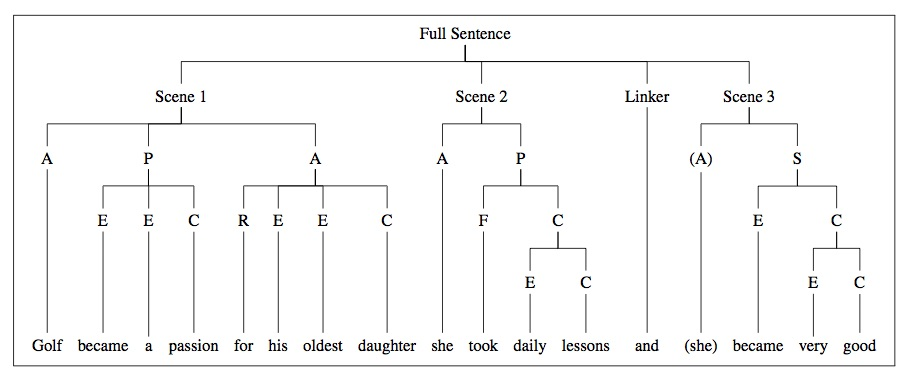
\includegraphics[width=1\textwidth]{ucca-tree.jpg}
    \caption{UCCA Tree with scenes}
    \label{ucca-tree}
\end{figure*}

%As you can see 
As can be seen
in Figure~\ref{ucca-tree}, the UCCA annotation results in a tree structure where each leaf is linked to
a word in the sentence at the bottom. A scene must contain a process (P) or a state (S). It can also contain
participants (A) and it can be linked to other scenes by a linker (Linker). Participants, processes and states can be
further analysed into elaborators (E), centres (C) and relators (R). These labels are very 
%high level 
high-level 
and relate to
cognitive concepts which should remain stable across languages.  

The fact that in UCCA
the labels are cognitive concepts and that they are linked directly to words
are both advantages 
when considering which semantic formalism is appropriate for machine translation evaluation.

One of such alternative formalisms is
Abstract Meaning Representation 
%%% Macro broken?
%(AMR; \inparcite{banarescu2013amr}). 
\cite{banarescu2013amr}. 
AMR is being actively developed with 
%the view to 
a view towards
using it as a way of generating 
translations but AMR graphs are not aligned to the words in the sentences. Having more abstract semantic structures 
makes the link between source words, target words, and structures more complex and potentially less useful. 
Furthermore, AMR  has been developed mainly with English in mind, and it remains
to be seen how universal AMR graphs are. See
\shortcite{amr:interlingua:lrec:2014} for first observations of divergences
between English 
%vs.
vs.\ 
Chinese and
Czech AMRs.

Another possible semantic framework for this kind of MT evaluation is Semantic
Role Labelling 
%(SRL; \inparcite{palmer2010semantic}).
\cite{palmer2010semantic}.
SRL has been used in a human translation metric called HMEANT~\cite{lo2011structured}. 
HMEANT uses semantic role labels
to measure how much of the “who, why, when,
where” has been preserved in translation. Annotators are instructed to identify verbs as
heads of semantic frames. Then they attach role
fillers to the heads and finally they align heads
and role fillers in the candidate translation with
those in a reference translation. Using SRL for evaluating SMT has a number of
disadvantages as explored by
\shortcite{birch-EtAl:2013:WMT} for German, \shortcite{bojar:wu:ssst:2012} for
Czech and by \shortcite{chuchunkov-tarelkin-galinskaya:2014:SSST-8} for Russian.
The most important drawbacks are as follows:
\begin{itemize}
\item SRL frames are based around a verb which is particularly problematic for
copular verbs and  when verbs are translated correctly as nouns or correctly
omitted (the verb ``to be'' in some Russian constructions).
\item SRL frames do not cover the entire source sentence and the semantic structure is
therefore not completely defined, importantly links between frames are not
considered and prepositional phrases which attach to nouns are not marked.
\item Even considering a limited set of eleven roles (agent, patient,
experiencer, locative etc.) is problematic because we cannot assume that these roles will 
 remain stable across different languages. 
 When looking at an automatically parsed  English-Chinese  parallel corpora,
 it was shown that 8.7\% of the arguments do not preserve their semantic roles~\cite{fung2006automatic}. 
\end{itemize}

UCCA provides universal semantic structures which 
%has 
have
a minimal set of labels. It provides a complete semantic tree which does not rely on syntactic heads and the semantic structure is grounded directly to the words in the sentence. 
 Even though the set of UCCA labels are fairly restricted,  nevertheless they allow us to determine the most important components of the graph (for example it defines centres and linkers which would be likely to carry more weight than elaborators), and we can use this to better calculate the score. 
We think that UCCA is the
most promising representation for evaluating translation. 
}

\section{Conclusion}

%\section*{Acknowledgments}

%Do not number the acknowledgment section.
%This section should not be presented for the submission version.

\bibliography{main}
\bibliographystyle{acl2016}


\end{document}
